
\section{Expérimentations}

Ces expérimentations comportent trois parties. La première partie se concentre
sur le comportement de \LSEQ dans les cas extrêmes. Les mesures capturent
l'effet d'un grand nombre d'insertions sur la taille des identifiants. Les
documents sont créés artificiellement selon différents comportements d'édition.
L'analyse s'effectue étape par étape afin de mettre en lumière la contribution
de chacun des composants de \LSEQ. En particulier, ces expérimentations ont pour
but de valider la complexité spatiale présentée à la section~\ref{sec:proposal}.
A ce titre, le système d'expérimentations est simple et n'implique qu'un seul
utilisateur. En d'autres termes, il n'y a pas de concurrence.


La seconde partie des expérimentations vise à simuler l'édition de documents à
plusieurs utilisateurs afin de mettre en valeur l'importance d'un choix de
sous-stratégies commun à tous les utilisateurs.

La troisième partie montre le comportement de \LSEQ face à Logoot sur des pages
Wikipedia (i.e. éditées par des humains mais sans concurrence) possédant
différents comportements d'édition.

Les expérimentations se concentre principalement sur les tailles des chemins
alloués. En effet, les disambiguators ont une complexité bornée par ceux-ci et
peuvent être drastiquement compressés.

Afin d'effectuer ces mesures, nous avons développé la structure de données \LSEQ
en Java dont les sources sont disponibles sur la plate-forme
Github~\footnote{\url{https://github.com/Chat-Wane/LSEQ}}. Le simulateur
d'édition impliquant de la concurrence est également disponible sur la
plate-forme
Github~\footnote{\url{https://github.com/Chat-Wane/HumbleSimulator}}.


\subsubsection{Simulations sans concurrence}

\begin{figure*}
  \centering
  \subfloat[Référentiel Logoot]
  [\label{fig:logoot}Logoot comme stratégie d'allocation référentielle.]
  {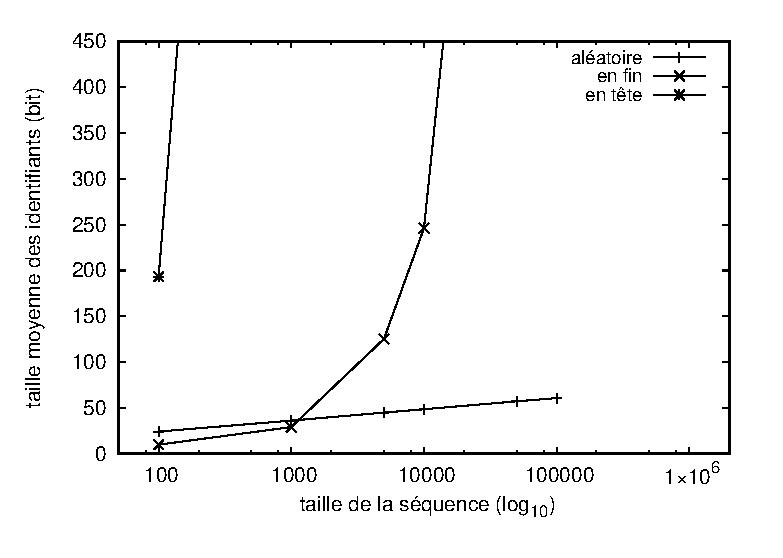
\includegraphics[width=0.48\textwidth]{./img/lseq/logoot.eps}}
  \hspace{10pt}
  \subfloat[Alternance de stratégies]
  [\label{fig:robin}Alternance de stratégie d'allocation antagonistes.]
  {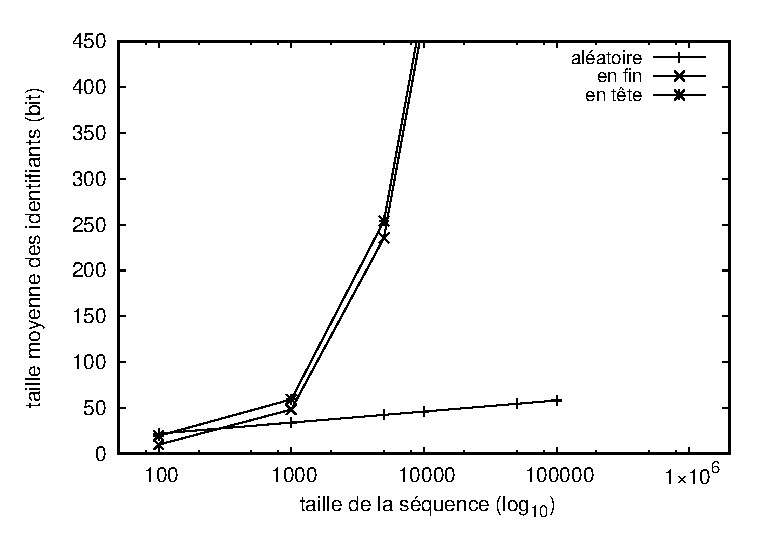
\includegraphics[width=0.48\textwidth]{./img/lseq/robin.eps}}
  \caption{Résultat des expérimentations impliquant une structure d'arbre avec
    arité constante.}
\end{figure*}

\begin{asparadesc}
\item [Objectif:] Montrer que la stratégie impliquant la structure d'arbre dont
  l'arité est constante avec une stratégie adapté à l'édition monotone en fin
  possède une complexité spatiale linéaire lorsque l'édition est monotone,
  logarithmique lorsque l'édition est aléatoire.
\item [Description:] Les mesures concernent la taille moyenne (en bits) des
  chemins alloués pour les identifiants. Les mesures sont effectuées à 100,
  1000, 5000, 10000, 50000, 100000 insertions dans la séquence. Les chemins sont
  alloués dans un arbre dont l'arité est constante ($2^{10}$). La stratégie
  d'allocation examinée est adaptée à l'édition en fin. Ce système correspond à
  aux composants de Logoot.
\item [Résultat:] La figure~\ref{fig:logoot} présente le nombre d'insertions sur
  l'axe des abscisses (avec une échelle logarithmique en base décimale). L'axe
  des ordonnées correspondent à la taille moyenne des identifiants (en
  bits). Comme attendu, la taille moyenne des identifiants augmente lors de l'
  insertion d'éléments dans la séquence. Lors de l'édition aléatoire,
  l'augmentation de taille des identifiants est logarithmique. Lors de l'édition
  monotone, l'augmentation est linéaire. Toutefois, l'édition en tête est
  extrêmement coûteuse. L'édition en fin reste acceptable en comparaison de
  l'édition en tête, mais l'augmentation linéaire de la taille des identifiants 
  conduirait inéluctablement à un coûteux \emph{garbage collect}.
\item [Explication:] L'édition en tête et en fin ont tendance à déséquilibrer
  une branche de l'arbre stockant les identifiants. La stratégie d'allocation
  étant spécifiquement adapté à l'édition en fin, elle réserve des branches en
  fin d'arbre en allouant les branches les plus à gauche. Hélas, la même
  stratégie avec comportement d'édition en opposition conduit à une augmentation
  rapide de la profondeur de l'arbre. Dans le pire cas, la taille totale des
  identifiants est de complexité $O(nb_insert^2)$. Pour de similaires raisons,
  l'édition à des positions aléatoires conduit à une augmentation logarithmique
  car la structure d'arbre est équilibrée.
\end{asparadesc}

\begin{figure*}
  \centering
  \subfloat[Augmentation de l'espace d'allocation]
  [\label{fig:double}Augmentation de l'espace d'allocation en fonction de 
  la profondeur de l'arbre.]
  {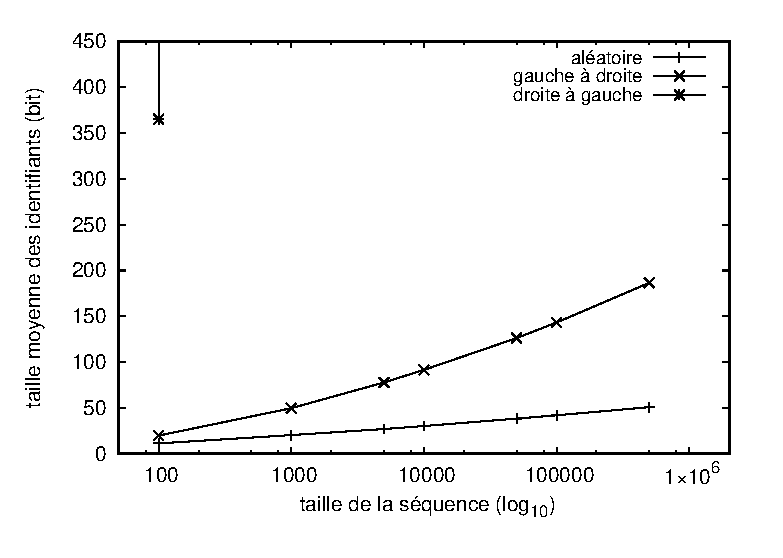
\includegraphics[width=0.48\textwidth]{./img/lseq/double.eps}}
  \hspace{10pt}
  \subfloat[Alternance et augmentation de l'espace d'allocation]
  [\label{fig:lseq}\LSEQ comme combinaison de l'alternance et de l'augmentation.]
  {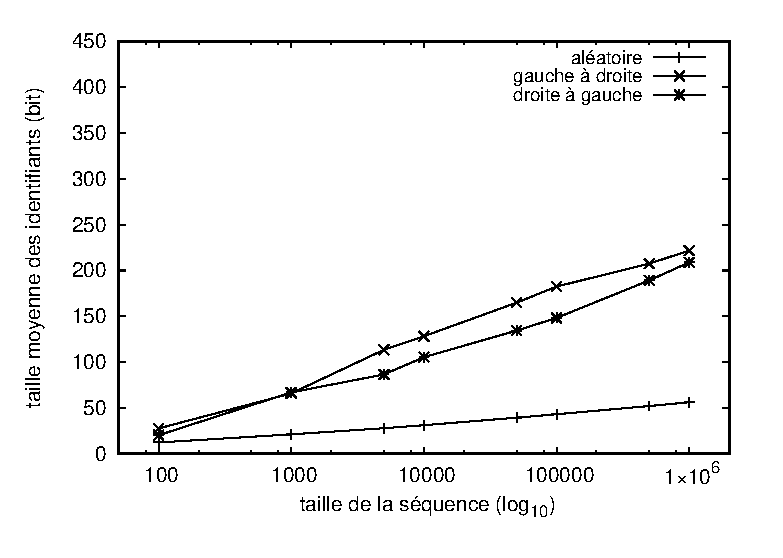
\includegraphics[width=0.48\textwidth]{./img/lseq/lseq.eps}}
\end{figure*}


\subsubsection{Simulations avec concurrence}

\begin{figure*}
  \centering
  \subfloat[Utilisateur unique]
  [\label{fig:one}Augmentation de l'espace d'allocation en fonction de 
  la profondeur de l'arbre.]
  {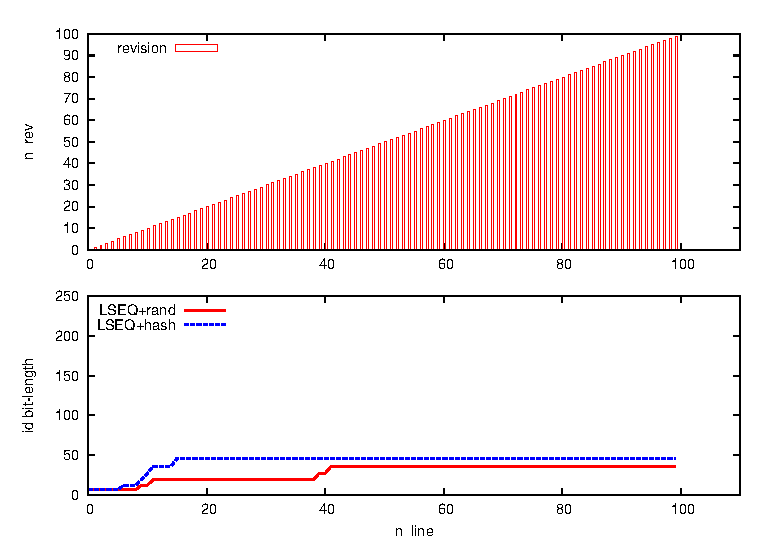
\includegraphics[width=0.48\textwidth]{./img/lseq/oneuser.eps}}
  \hspace{10pt}
  \subfloat[Alternance et augmentation de l'espace d'allocation]
  [\label{fig:ten}\LSEQ comme combinaison de l'alternance et de l'augmentation.]
  {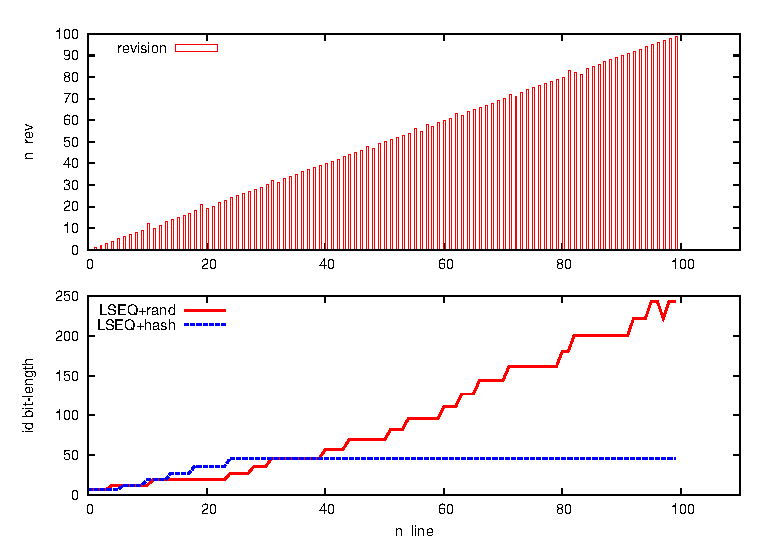
\includegraphics[width=0.48\textwidth]{./img/lseq/tenusers.eps}}
  \caption{Spectre de document artificiel générés par insertion répétée de caractère
  en queue.}
\end{figure*}


\subsubsection{Simulations sur traces Wikipedia}

\begin{figure*}
  \centering
  \subfloat[Comportement d'édition attendu]
  [\label{fig:compliant}Le comportement d'édition correspond aux attentes
  de la stratégie d'allocation]
  {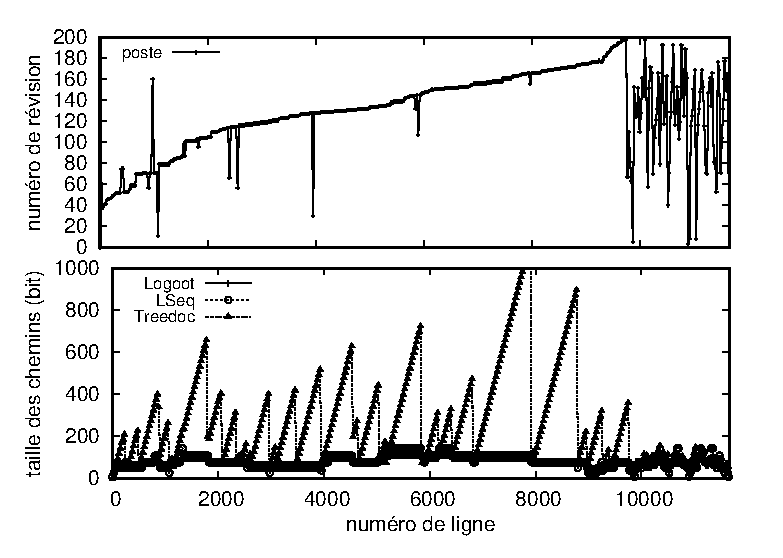
\includegraphics[width=0.48\textwidth]{./img/lseq/poste.eps}}
  \hspace{10pt}
  \subfloat[Comportement d'édition inattendu]
  [\label{fig:motivating}Le comportement d'édition va à l'encontre des attentes
  de la stratégie d'allocation]
  {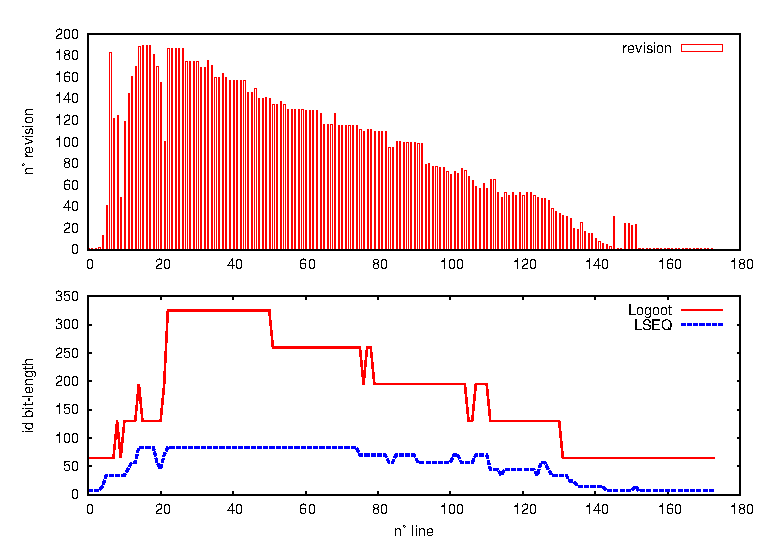
\includegraphics[width=0.48\textwidth]{./img/lseq/didyouknow.eps}}
  \caption{\label{fig:allocation}Spectre de document Wikipedia sous différent
    comportements d'édition antagonistes. La figure du haut représente la
    révision à laquelle la ligne a été inséré, i.e., sa date de naissance.  La
    figure du bas représente la taille de l'identifiant associé à chaque ligne.}
\end{figure*}

%%% Local Variables:
%%% mode: latex
%%% TeX-master: "../../paper"
%%% End:
